\chapter{Appendix}
\label{cha:Appendix}

\section{Code Repository}

The code repository is publically availible on GitHub:

\href{https://github.com/geschnee/carsim-rl-cnn}{carsim-rl-cnn}

The readme file contains instructions on how to install and run the code.

\section{Most successful model}

The most successful model is publically availible on Huggingface:

\href{https://huggingface.co/geschnee/carsim-rl-cnn}{carsim-rl-cnn}

\href{https://huggingface.co/geschnee/carsim-rl-cnn/blob/main/models/hardDistanceMixedLight.zip}{hardDistanceMixedLight.zip}

The episode recordings for question 3 are also hosted there.

\section{Experiments for finding hyperparameters - Configuration files}
\label{cha:experiment_configs}

how to run a specific config? link readme

\subsection{Reward functions capability check}
The used configs are the following:
\begin{itemize}
    \item \href{https://github.com/geschnee/carsim-rl-cnn/tree/main/python/cfg/ppo_rewardFunction_capability_check_orientationReward.yaml}{ppo\_rewardFunction\_capability\_check\_orientationReward.yaml}
    \item \href{https://github.com/geschnee/carsim-rl-cnn/tree/main/python/cfg/ppo_rewardFunction_capability_check_distanceReward.yaml}{ppo\_rewardFunction\_capability\_check\_distanceReward.yaml}
    \item \href{https://github.com/geschnee/carsim-rl-cnn/tree/main/python/cfg/ppo_rewardFunction_capability_check_velocityReward.yaml}{ppo\_rewardFunction\_capability\_check\_velocityReward.yaml}
    \item \href{https://github.com/geschnee/carsim-rl-cnn/tree/main/python/cfg/ppo_rewardFunction_capability_check_eventReward.yaml}{ppo\_rewardFunction\_capability\_check\_eventReward.yaml}
\end{itemize}


\subsection{Most Successful Policy Configuration}
\label{cha:most_successful_config}

The training config of the model for the final evaluations is availible on GitHub:
\href{https://github.com/geschnee/carsim-rl-cnn/tree/main/python/cfg/hardDistanceMixedLight.yaml}{hardDistanceMixedLight.yaml}

\section{Example Video Files}
\label{cha:example_videos}

Video Files are availible on Github:
\href{https://github.com/geschnee/carsim-rl-cnn/tree/main/python/results/example_videos}{example\_videos}

\subsection{Video Files with FourWheelJetBot}

\paragraph{Collisions}
\label{sec:fourwheel_collisions}

The collisions are generally more severe for the FourWheelJetBot:

\begin{itemize}
    \item \href{https://huggingface.co/geschnee/carsim-rl-cnn/blob/main/example_videos_FourWheelJetbot/hard_standard_FourWheelJetBot_env_0_video_1_topview.gif}{example\_videos/hard\_standard\_FourWheelJetBot\_env\_0\_video\_1\_topview.gif}
    \item \href{https://huggingface.co/geschnee/carsim-rl-cnn/blob/main/example_videos_FourWheelJetbot/hard_standard_FourWheelJetBot_env_0_video_2_topview.gif}{example\_videos/hard\_standard\_FourWheelJetBot\_env\_0\_video\_2\_topview.gif}
\end{itemize}


\section{All Tracks}

\begin{figure}
    \centering
    \subfigure[easyBlueFirst]{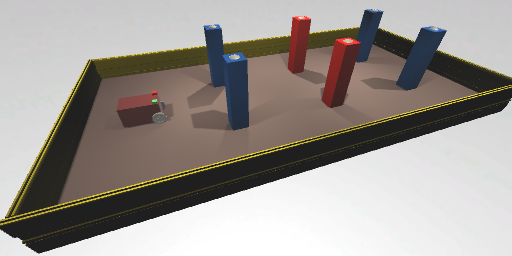
\includegraphics[width=0.3\textwidth]{Bilder/image_printer_images/tracks/MapType.easyBlueFirst.png}}\qquad
    \subfigure[easyRedFirst]{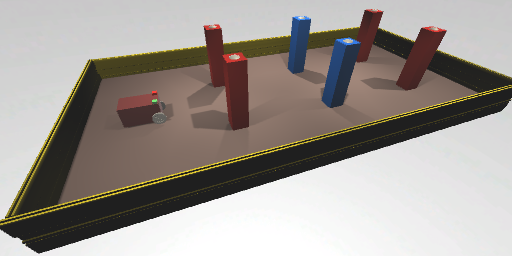
\includegraphics[width=0.3\textwidth]{Bilder/image_printer_images/tracks/MapType.easyRedFirst.png}}\\
    \subfigure[mediumBlueFirstLeft]{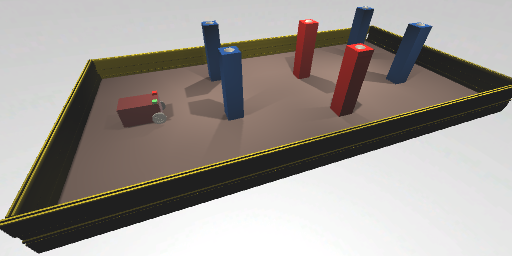
\includegraphics[width=0.2\textwidth]{Bilder/image_printer_images/tracks/MapType.mediumBlueFirstLeft.png}}\qquad
    \subfigure[mediumBlueFirstRight]{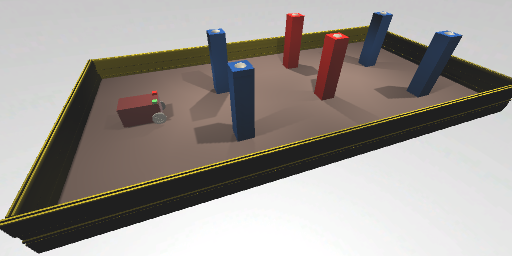
\includegraphics[width=0.2\textwidth]{Bilder/image_printer_images/tracks/MapType.mediumBlueFirstRight.png}}\qquad
    \subfigure[mediumRedFirstLeft]{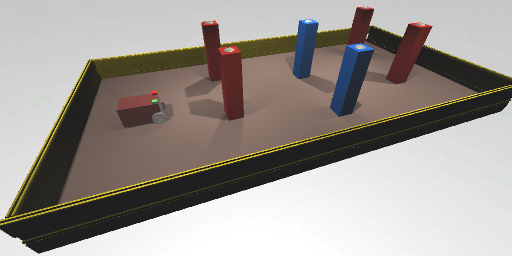
\includegraphics[width=0.2\textwidth]{Bilder/image_printer_images/tracks/MapType.mediumRedFirstLeft.png}}\qquad
    \subfigure[mediumRedFirstRight]{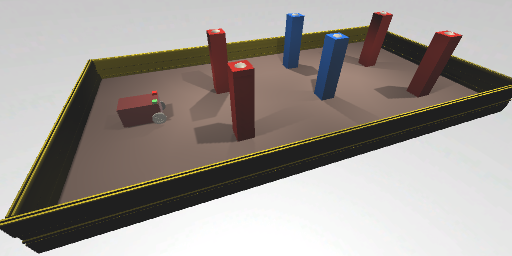
\includegraphics[width=0.2\textwidth]{Bilder/image_printer_images/tracks/MapType.mediumRedFirstRight.png}}\\
    \subfigure[hardBlueFirstLeft]{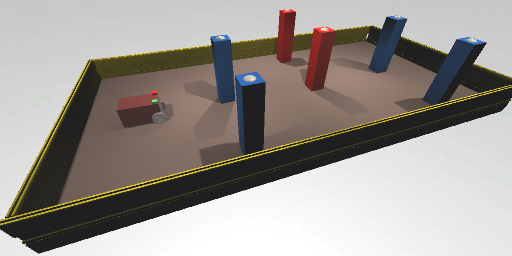
\includegraphics[width=0.2\textwidth]{Bilder/image_printer_images/tracks/MapType.hardBlueFirstLeft.png}}\qquad
    \subfigure[hardBlueFirstRight]{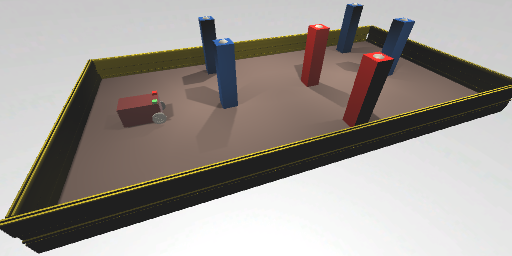
\includegraphics[width=0.2\textwidth]{Bilder/image_printer_images/tracks/MapType.hardBlueFirstRight.png}}\qquad
    \subfigure[hardRedFirstLeft]{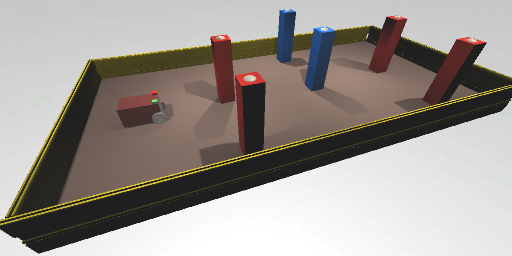
\includegraphics[width=0.2\textwidth]{Bilder/image_printer_images/tracks/MapType.hardRedFirstLeft.png}}\qquad
    \subfigure[hardRedFirstRight]{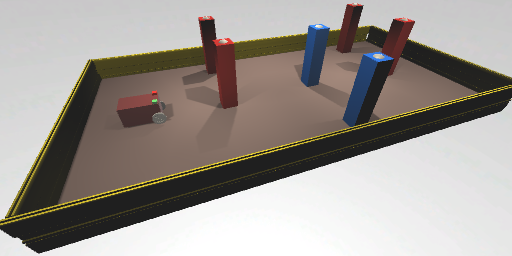
\includegraphics[width=0.2\textwidth]{Bilder/image_printer_images/tracks/MapType.hardRedFirstRight.png}}\\
    \caption{All tracks}
    \label{fig:all_tracks}
\end{figure}


\section{Pseudocode}

TODO pseudocde für basic\_eval\_algorithm?

\renewcommand{\thepseudonum}{\roman{pseudonum}}
\begin{pseudocode}{Collect Data}{ }
    \COMMENT{Fill RolloutBuffer with samples obtained by current model}\\

    \PROCEDURE{CollectData}{trainingMapType, trainingLightSetting}
    num\_steps \GETS 0\\
    num\_episodes \GETS 0\\
    num\_succesful\_episodes \GETS 0\\

    RolloutBuffer.\CALL{Reset}{trainingMapType, trainingLightSetting}\\
    Env.\CALL{Reset}{}\\
    \WHILE RolloutBuffer.\CALL{NotFull}{} \DO
    \BEGIN
    obs \GETS Env.\CALL{GetObservation}{}\\
    action \GETS Model.\CALL{GetAction}{obs}\\
    reward \GETS Env.\CALL{Step}{action}\\
    num\_steps \GETS num\_steps + 1\\
    \CALL{AddToRolloutBuffer}{obs, action, reward}\\
    \IF Env.\CALL{IsFinished}{} \THEN
    \BEGIN
    num\_episodes \GETS num\_episodes + 1\\
    \IF Env.\CALL{FinishedSuccessfully}{} \THEN
    \BEGIN
    num\_succesful\_episodes \GETS num\_succesful\_episodes + 1\\
    \END\\
    Env.\CALL{Reset}{trainingMapType, trainingLightSetting}\\
    \END\\
    \END\\

    rollout\_success\_rate \GETS \frac{num\_succesful\_episodes}{num\_episodes}\\

    \IF rollout\_success\_rate >= best\_rollout\_success\_rate \THEN
    \BEGIN
    best\_success\_rate \GETS rollout\_success\_rate\\
    Model.\CALL{SaveToFile}{}\\
    best\_model \GETS Model\\
    \END\\


    \RETURN{num\_steps}
    \ENDPROCEDURE
    \label{pseudocode:collect_data}
\end{pseudocode}

\renewcommand{\thepseudonum}{\roman{pseudonum}}
\begin{pseudocode}{Train Model}{ }
    \COMMENT{Sample from replay buffer and update the model based on the loss}\\

    \PROCEDURE{TrainModel}{}
    amount\_of\_batches \GETS \frac{rollout\_buffer\_size}{batch\_size}\\
    \FOR i \GETS 0 \TO n\_epochs \DO
    \BEGIN
    RolloutBuffer.\CALL{Shuffle}{}\\
    RolloutBuffer.\CALL{CreateBatches}{batch\_size}\\
    \FOR m \GETS 0 \TO amount\_of\_batches \DO
    \BEGIN
    batch \GETS RolloutBuffer.\CALL{GetBatch}{m}\\
    loss \GETS \CALL{ComputeLoss}{batch}\\
    Model.\CALL{Backpropagate}{loss}\\
    Optimizer.\CALL{Step}{}\\
    \END\\
    \END
    \ENDPROCEDURE
    \label{pseudocode:train_model}
\end{pseudocode}

\section{Neural Network Architecture}

\begin{figure}
    \centering
    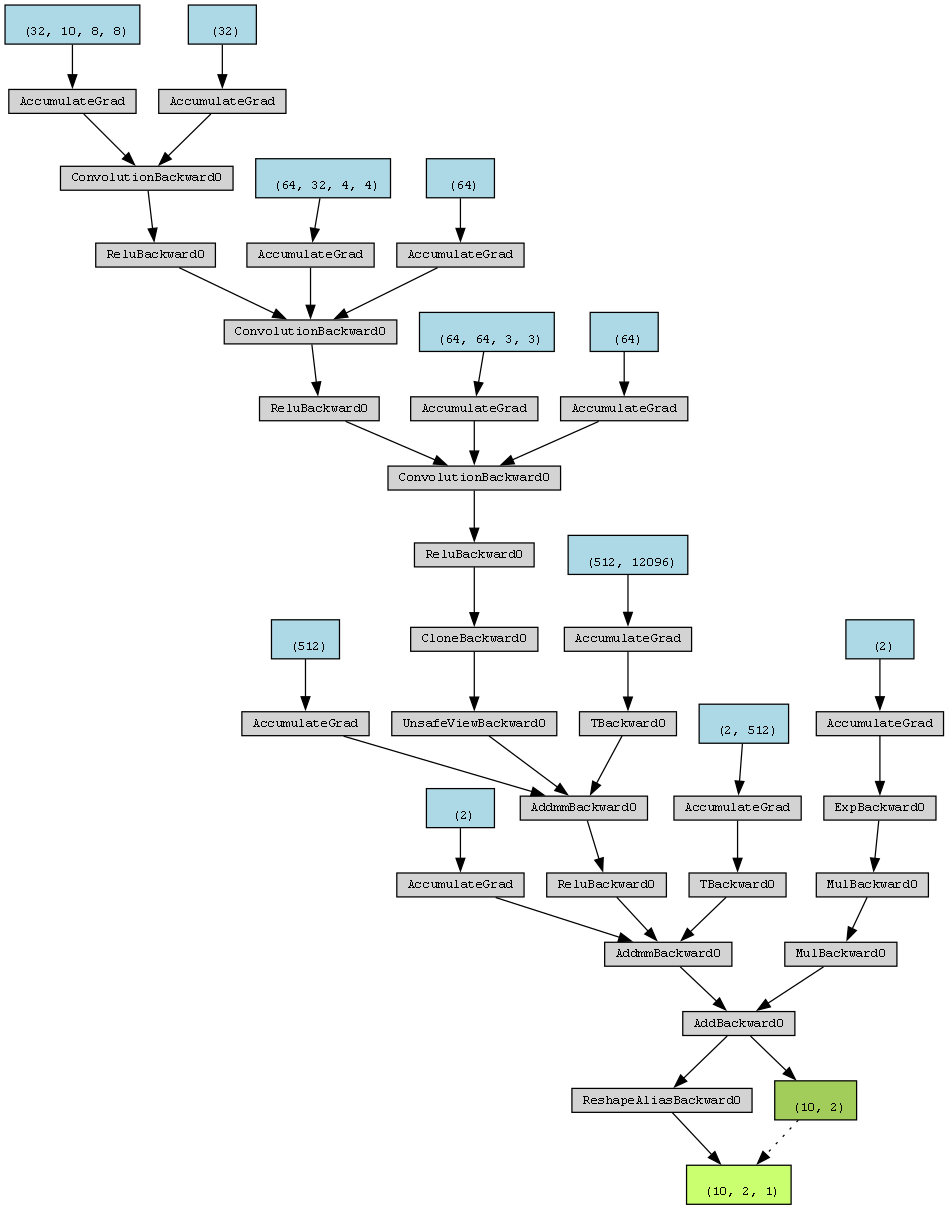
\includegraphics[width=0.7\textwidth]{Bilder/action_graph.png}
    \caption{Neural Network Architecture Action Head}
    \label{fig:action_graph}
\end{figure}

\begin{figure}
    \centering
    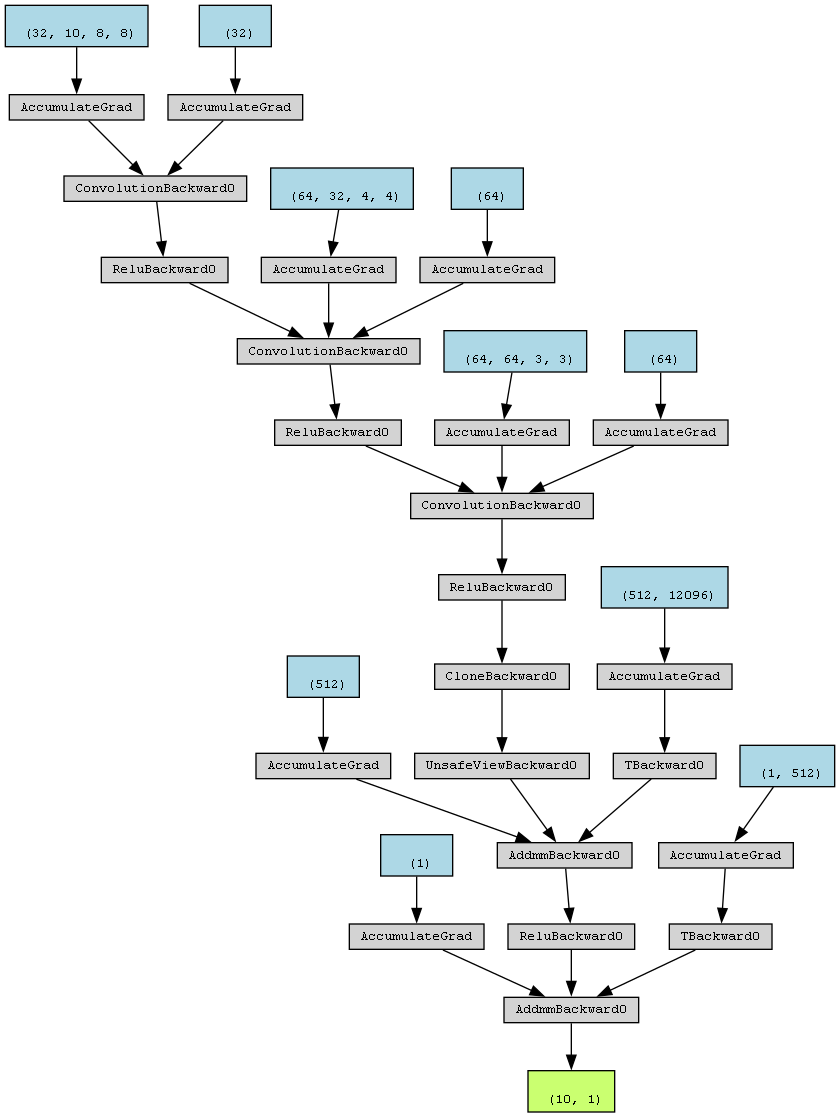
\includegraphics[width=0.7\textwidth]{Bilder/value_graph.png}
    \caption{Neural Network Architecture Value Head}
    \label{fig:value_graph}
\end{figure}


\section{Eval Model Track}
\renewcommand{\thepseudonum}{\roman{pseudonum}}
\begin{pseudocode}{Generate Map and Rotation Combinations}{ }

    \PROCEDURE{generate\_map\_and\_rotations}{difficulty, n\_eval\_episodes, env}

    rotationMode \GETS env.\CALL{getSpawnMode}{}\\
    rotation\_range\_min, rotation\_range\_max \GETS Spawn.\CALL{getRotationRange}{rotationMode}\\

    range\_width \GETS rotation\_range\_max - rotation\_range\_min\\
    rotations \GETS []\\

    \IF n\_eval\_episodes == 1 \THEN
    rotations.\CALL{append}{(rotation\_range\_min + range\_width)/2}\\
    \ELSE
    \BEGIN
    step \GETS range\_width / (n\_eval\_episodes -1)\\
    \FOR i \GETS 0 \TO n\_eval\_episodes - 1 \DO
    \BEGIN
    rotations.\CALL{append}{rotation\_range\_min + i * step}\\
    \END\\
    \END\\

    track\_numbers \GETS MapType.\CALL{getAllTracknumbersOfDifficulty}{difficulty}\\
    tracks \GETS []\\
    \FOR i \GETS 0 \TO n\_eval\_episodes - 1 \DO
    \BEGIN
    tracks.\CALL{append}{i \mod \CALL{len}{track\_numbers}}\\
    \END\\

    combinations \GETS []\\
    \FOR i \GETS 0 \TO n\_eval\_episodes - 1 \DO
    \BEGIN
    combinations.\CALL{append}{(tracks[i], rotations[i])}\\
    \END\\

    \RETURN{combinations}
    \ENDPROCEDURE
    \label{fig:generate_track_rotation}
\end{pseudocode}



\section{Replay on JetBot}

\subsection{Installation instructions for executing replays on the Jetbot}

The replays are executed on NVIDIA Jetbot hardware. The test does not make use of jetbot specific hardware and software features such as the jetbot camera. The test runs on the jetbot's standard ubuntu installation. Instructions for the installation and execution of the replay test are availible in the \href{https://github.com/geschnee/carsim-rl-cnn/blob/main/replays_on_jetbot.md}{replays\_on\_jetbot.md file} in the code repository.


\renewcommand{\thepseudonum}{\roman{pseudonum}}
\begin{pseudocode}{Record Episode}{ }
    \COMMENT{Record episode}\\

    \PROCEDURE{record\_episode}{policy, env, directory}

    env.\CALL{RESET}{}\\

    sampled\_actions \GETS [] \\
    infer\_obsstrings \GETS [] \\
    step\_obsstrings \GETS [] \\

    done \GETS \FALSE\\

    \WHILE ! done \DO
    \BEGIN
    obs, obsstring \GETS env.\CALL{GetObservation}{}\\
    action \GETS policy.\CALL{Infer}{obs}\\

    step\_obsstring, done \GETS env.\CALL{step}{action}\\

    infer\_obsstrings.\CALL{append}{obsstring}\\
    step\_obsstrings.\CALL{append}{step\_obsstring}\\
    sampled\_actions.\CALL{append}{action}\\
    \END\\

    \FOR i \GETS 0 \TO len(step\_obsstrings) \DO
    \CALL{SaveToFile}{step\_obsstrings[i], directory + ''/step\_image'' + i + ''.png''}\\
    \FOR i \GETS 0 \TO len(infer\_obsstrings) \DO
    \CALL{SaveToFile}{infer\_obsstrings[i], directory + ''/infer\_image'' + i + ''.png''}\\
    \FOR i \GETS 0 \TO len(sampled\_actions) \DO
    \CALL{SaveToFile}{sampled\_actions[i], directory + ''/sampled\_action'' + i + ''.npy''}\\


    \ENDPROCEDURE
    \label{pseudocode:record_episode}
\end{pseudocode}

\renewcommand{\thepseudonum}{\roman{pseudonum}}
\begin{pseudocode}{Replay Episode}{ }
    \COMMENT{Replay episode and record processing + inference time}\\

    \PROCEDURE{replay\_episode}{ policy, env, directory}

    recorded\_episode\_length \GETS \CALL{LoadRecordedEpisodeLength}{directory}\\
    recorded\_actions \GETS \CALL{LoadRecordedActions}{directory}\\
    infer\_obs\_unity\_images \GETS \CALL{LoadInferImages}{directory}\\
    step\_obs\_unity\_images \GETS \CALL{LoadStepImages}{directory}\\

    reproduce\_times \GETS [] \\

    replay\_time\_start \GETS \CALL{TIME}{}\\

    \FOR i \GETS 0 \TO recorded\_episode\_length \DO
    \BEGIN
    obs \GETS \CALL{ProcessImage}{env, infer\_obs\_unity\_images[i]}\\
    action \GETS policy.\CALL{Infer}{obs}\\
    reproduce\_times.\CALL{append}{\CALL{TIME}{} - replay\_time\_start}\\

    \CALL{AssertClose}{action, recorded\_actions[i]}\\

    replay\_time\_start \GETS \CALL{TIME}{}\\

    \CALL{ProcessImage}{env, step\_obs\_unity\_images[i]}\\
    \END\\
    \RETURN{reproduce\_times}
    \ENDPROCEDURE

    \label{pseudocode:replay_episode}
\end{pseudocode}

